%!TEX TS-program = xelatex
\documentclass[12pt, a4paper, oneside]{article}

\usepackage{amsmath,amsfonts,amssymb,amsthm,mathtools}  % пакеты для математики

\usepackage[english, russian]{babel} % выбор языка для документа
\usepackage[utf8]{inputenc} % задание utf8 кодировки исходного tex файла
\usepackage[X2,T2A]{fontenc}        % кодировка

\usepackage{fontspec}         % пакет для подгрузки шрифтов
\setmainfont{Linux Libertine O}   % задаёт основной шрифт документа

\usepackage{unicode-math}     % пакет для установки математического шрифта
\setmathfont[math-style=upright]{Neo Euler} % шрифт для математики

% Конкретный символ из конкретного шрифта
% \setmathfont[range=\int]{Neo Euler}


% Конкретный символ из конкретного шрифта
% \setmathfont[range=\int]{Neo Euler}

%%%%%%%%%% Работа с картинками %%%%%%%%%
\usepackage{graphicx}                  % Для вставки рисунков
\usepackage{graphics}
\graphicspath{{images/}{pictures/}}    % можно указать папки с картинками
\usepackage{wrapfig}                   % Обтекание рисунков и таблиц текстом

%%%%%%%%%%%%%%%%%%%%%%%% Графики и рисование %%%%%%%%%%%%%%%%%%%%%%%%%%%%%%%%%
\usepackage{tikz, pgfplots}  % язык для рисования графики из latex'a

%%%%%%%%%% Гиперссылки %%%%%%%%%%
\usepackage{xcolor}              % разные цвета

\usepackage{hyperref}
\hypersetup{
	unicode=true,           % позволяет использовать юникодные символы
	colorlinks=true,       	% true - цветные ссылки, false - ссылки в рамках
	urlcolor=blue,          % цвет ссылки на url
	linkcolor=red,          % внутренние ссылки
	citecolor=green,        % на библиографию
	pdfnewwindow=true,      % при щелчке в pdf на ссылку откроется новый pdf
	breaklinks              % если ссылка не умещается в одну строку, разбивать ли ее на две части?
}


\usepackage{todonotes} % для вставки в документ заметок о том, что осталось сделать
% \todo{Здесь надо коэффициенты исправить}
% \missingfigure{Здесь будет Последний день Помпеи}
% \listoftodos --- печатает все поставленные \todo'шки

\usepackage[paper=a4paper, top=20mm, bottom=15mm,left=20mm,right=15mm]{geometry}
\usepackage{indentfirst}       % установка отступа в первом абзаце главы

\usepackage{setspace}
\setstretch{1.15}  % Межстрочный интервал
\setlength{\parskip}{4mm}   % Расстояние между абзацами
% Разные длины в латехе https://en.wikibooks.org/wiki/LaTeX/Lengths


\usepackage{xcolor} % Enabling mixing colors and color's call by 'svgnames'

\definecolor{MyColor1}{rgb}{0.2,0.4,0.6} %mix personal color
\newcommand{\textb}{\color{Black} \usefont{OT1}{lmss}{m}{n}}
\newcommand{\blue}{\color{MyColor1} \usefont{OT1}{lmss}{m}{n}}
\newcommand{\blueb}{\color{MyColor1} \usefont{OT1}{lmss}{b}{n}}
\newcommand{\red}{\color{LightCoral} \usefont{OT1}{lmss}{m}{n}}
\newcommand{\green}{\color{Turquoise} \usefont{OT1}{lmss}{m}{n}}

\usepackage{titlesec}
\usepackage{sectsty}
%%%%%%%%%%%%%%%%%%%%%%%%
%set section/subsections HEADINGS font and color
\sectionfont{\color{MyColor1}}  % sets colour of sections
\subsectionfont{\color{MyColor1}}  % sets colour of sections

%set section enumerator to arabic number (see footnotes markings alternatives)
\renewcommand\thesection{\arabic{section}.} %define sections numbering
\renewcommand\thesubsection{\thesection\arabic{subsection}} %subsec.num.

%define new section style
\newcommand{\mysection}{
	\titleformat{\section} [runin] {\usefont{OT1}{lmss}{b}{n}\color{MyColor1}} 
	{\thesection} {3pt} {} } 


%	CAPTIONS
\usepackage{caption}
\usepackage{subcaption}
%%%%%%%%%%%%%%%%%%%%%%%%
\captionsetup[figure]{labelfont={color=Turquoise}}

\pagestyle{empty}


%%%%%%%%%% Свои команды %%%%%%%%%%
\usepackage{etoolbox}    % логические операторы для своих макросов

% Все свои команды лучше всего определять не по ходу текста, как это сделано в этом документе, а в преамбуле!

% Одно из применений - уничтожение какого-то куска текста!
\newbool{answers}
%\booltrue{answers}
\boolfalse{answers}

\begin{document}

\section*{Самостоятельная работа. Вариант I}

\textbf{Решите все задания. Все ответы должны быть обоснованы. Все решения должны быть чётко приведены для каждого пункта. Рисунки должны быть чёткими, понятными. Все лении должны быть подписаны. Списывание карается обнулением баллов. Удачи!}

\subsection*{[5] Задача 1 }

Дайте ответы на вопросы, приведённые ниже. 

\begin{enumerate}
	\item  
	
	\hspace{2cm} \textbf{Да}  \hspace{4cm} \textbf{Нет} 
		
	\item 
	
	\hspace{2cm} \textbf{Да}  \hspace{4cm} \textbf{Нет} 
		
	\item 
	
	\hspace{2cm} \textbf{Да}  \hspace{4cm} \textbf{Нет} 
		
	\item 	
	
	\hspace{2cm} \textbf{Да}  \hspace{4cm} \textbf{Нет} 
	
	\item 
	
	\hspace{2cm} \textbf{Да}  \hspace{4cm} \textbf{Нет} 
	
	\item 
	
	\hspace{2cm} \textbf{Да}  \hspace{4cm} \textbf{Нет} 
		
	\item 
	
	\hspace{2cm} \textbf{Да}  \hspace{4cm} \textbf{Нет} 
	
	\item
	
	\hspace{2cm} \textbf{Да}  \hspace{4cm} \textbf{Нет} 
	 	
	\item
	
	\hspace{2cm} \textbf{Да}  \hspace{4cm} \textbf{Нет} 
	
	\item 
	
	\hspace{2cm} \textbf{Да}  \hspace{4cm} \textbf{Нет} 
	
	\item  	Хорошо, то не было вопросов про случайный лес.
	
	\hspace{2cm} \textbf{Да}  \hspace{4cm} \textbf{Нет} 
	
\end{enumerate}

\subsection*{[15] Задача 2}

На плоскости расположены колонии рыжих и чёрных муравьёв. Рыжих колоний три и они имеют координаты $(-1, 1)$, $(1, -1)$ и $(1, 1)$. Чёрных колоний одна и она имеет координаты $(0, 0)$.

\begin{enumerate}
	\item Поделите плоскость на «зоны влияния» рыжих и чёрных используя метод одного и трёх ближайших соседей.
	
	\item С помощью кросс-валидации с выкидыванием отдельных наблюдений выберите оптимальное число соседей $k$ перебрав $k \in \{1, 3 \}$. Целевой функцией является количество несовпадающих прогнозов.
\end{enumerate}


\subsection*{[5] Задача 3}

Объясните шутку: 

\begin{center}
	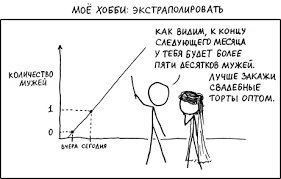
\includegraphics[scale=0.8]{memes.png}
\end{center}



\newpage 

\section*{Самостоятельная работа. Вариант II}

Решите все задания. Все ответы должны быть обоснованы. Все решения должны быть чётко приведены для каждого пункта. Рисунки должны быть чёткими, понятными. Все лении должны быть подписаны. 

\subsection*{Задача 1 }

Дайте ответ на вопросы, приведённые ниже. 

\begin{enumerate}
	\item  Переобученная модель может хорошо обрабатывать новые примеры. В машинном обучении всегда стараются как можно сильнее переобучить модель.
	
	\hspace{2cm} \textbf{Да}  \hspace{4cm} \textbf{Нет} 
	
	\item 
	
	\hspace{2cm} \textbf{Да}  \hspace{4cm} \textbf{Нет} 
	
	\item 
	
	\hspace{2cm} \textbf{Да}  \hspace{4cm} \textbf{Нет} 
	
	\item 	
	
	\hspace{2cm} \textbf{Да}  \hspace{4cm} \textbf{Нет} 
	
	\item 
	
	\hspace{2cm} \textbf{Да}  \hspace{4cm} \textbf{Нет} 
	
	\item 
	
	\hspace{2cm} \textbf{Да}  \hspace{4cm} \textbf{Нет} 
	
	\item 
	
	\hspace{2cm} \textbf{Да}  \hspace{4cm} \textbf{Нет} 
	
	\item
	
	\hspace{2cm} \textbf{Да}  \hspace{4cm} \textbf{Нет} 
	
	\item
	
	\hspace{2cm} \textbf{Да}  \hspace{4cm} \textbf{Нет} 
	
	\item 
	
	\hspace{2cm} \textbf{Да}  \hspace{4cm} \textbf{Нет} 
	
	\item  	«Математику уже затем учить надо, что она ум в порядок приводит» (Ломоносов)
	
	\hspace{2cm} \textbf{Да}  \hspace{4cm} \textbf{Нет} 
	
\end{enumerate}




\subsection*{Задача 3}

Объясните шутку: 

\begin{center}
	
\includegraphics[scale=0.3]{memes2.jpg}
\end{center}

\newpage 


\section*{Самостоятельная работа. Вариант III}

Решите все задания. Все ответы должны быть обоснованы. Все решения должны быть чётко приведены для каждого пункта. Рисунки должны быть чёткими, понятными. Все лении должны быть подписаны. 

\subsection*{Задача 1 }

Дайте ответ на вопросы, приведённые ниже.

\begin{enumerate}
	\item  
	
	\hspace{2cm} \textbf{Да}  \hspace{4cm} \textbf{Нет} 
	
	\item В задаче кластеризации есть размеченная выборка. Мы по ней пытаемся научить алгоритм разбираться где какой класс. В задаче классификации такой выборки нет. 
	
	\hspace{2cm} \textbf{Да}  \hspace{4cm} \textbf{Нет} 
	
	\item 
	
	\hspace{2cm} \textbf{Да}  \hspace{4cm} \textbf{Нет} 
	
	\item 	
	
	\hspace{2cm} \textbf{Да}  \hspace{4cm} \textbf{Нет} 
	
	\item 
	
	\hspace{2cm} \textbf{Да}  \hspace{4cm} \textbf{Нет} 
	
	\item 
	
	\hspace{2cm} \textbf{Да}  \hspace{4cm} \textbf{Нет} 
	
	\item 
	
	\hspace{2cm} \textbf{Да}  \hspace{4cm} \textbf{Нет} 
	
	\item
	
	\hspace{2cm} \textbf{Да}  \hspace{4cm} \textbf{Нет} 
	
	\item
	
	\hspace{2cm} \textbf{Да}  \hspace{4cm} \textbf{Нет} 
	
	\item 
	
	\hspace{2cm} \textbf{Да}  \hspace{4cm} \textbf{Нет} 
	
	\item У другой группы была задача с методом ближайших соседей. Жалко, что я не из неё.
		
	\hspace{2cm} \textbf{Да}  \hspace{4cm} \textbf{Нет} 
	
\end{enumerate}




\subsection*{Задача 3}

Объясните шутку: 

\begin{center}
	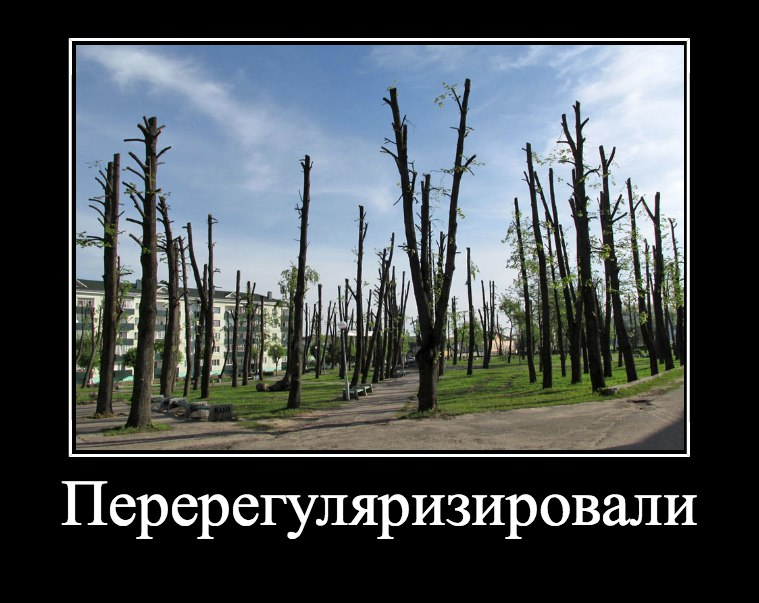
\includegraphics[scale=0.5]{memes3.jpg}
\end{center}


\end{document}



